\section{Methodology}\label{sec:metodo}

\subsection{Image Dataset}
We merged TrashNet~\cite{trashnet} (MIT license, white background) and the six equivalent classes of RealWaste~\cite{realwaste} (CC BY-NC-SA 4.0, real waste from a materials recovery facility): \ImgTotal{} images labeled by their authors (Fig.~\ref{fig:examples}). Mixing both sources avoids depending on a single background.

Exact duplicates were removed by pixel hash. Since both datasets contain several photos of the same object, a random split would leak information. We computed embeddings with a pretrained ResNet-50 and merged into connected components the same-source pairs with a cosine similarity of 0.88 or higher, a threshold chosen by inspecting real pairs. This yielded \ImgGroups{} groups, with \ImgInGroups{} images in groups of two or more. Each group was assigned as a whole to a 70/15/15 split, stratified by class and source (Table~\ref{tab:images}).

\begin{figure*}[t]
\centering
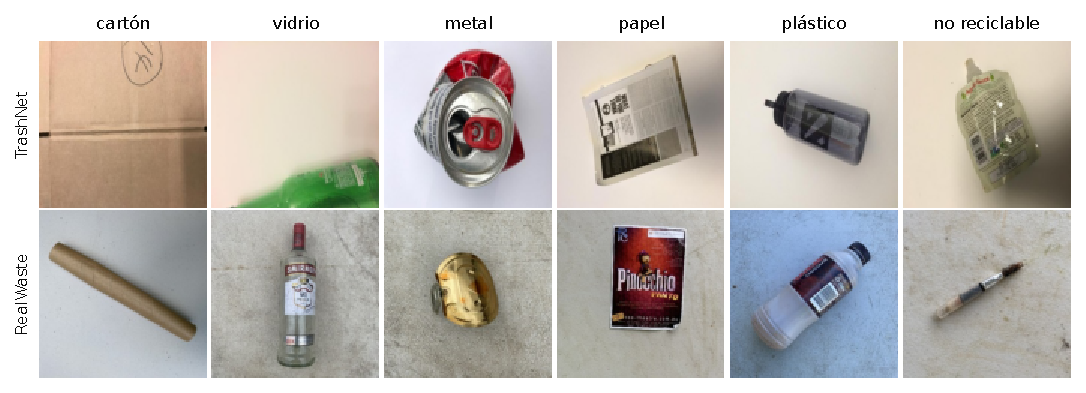
\includegraphics[width=0.76\textwidth]{dataset_examples.pdf}
\caption{Training examples by class and source. The background and the condition of the objects differ between the two datasets.}
\label{fig:examples}
\end{figure*}

\begin{table}[t]
\centering
\caption{Images per class and split}
\label{tab:images}
\begin{tabular}{lrrrr}
\toprule
Class & Train & Val. & Test & Total \\
\midrule
cardboard & 604 & 130 & 130 & 864 \\
glass & 642 & 138 & 138 & 918 \\
metal & 837 & 181 & 181 & 1199 \\
paper & 766 & 164 & 164 & 1094 \\
plastic & 980 & 211 & 210 & 1401 \\
non-recyclable & 441 & 96 & 95 & 632 \\
\textbf{Total} & 4270 & 920 & 918 & 6108 \\
\bottomrule
\end{tabular}

\end{table}

\subsection{Speech Dataset}
Two sources were combined. The first is a random sample of 12\,000 recordings from TUX~\cite{tux}, the course's class dataset, with a single speaker. The second is the Latin American OpenSLR 72, 73, and 74 corpora~\cite{openslr} (Colombia, Peru, and Puerto Rico, CC BY-SA 4.0). Everything was converted to 16\,kHz, 16-bit mono WAV, leading and trailing silence was trimmed, and clips of 0.7 to 12\,s were kept. Transcriptions were normalized to lowercase, without punctuation, over a 34-symbol alphabet that keeps accents, \emph{ü}, and \emph{ñ}. The result is \AudioTotal{} recordings and \AudioHours{} hours (Table~\ref{tab:audio}).

In OpenSLR, the same sentence is read by up to 94 people. One speaker per country and sex was held out for validation and another for testing, and every held-out sentence was removed from training, regardless of who read it. This control, together with the remaining recordings of the held-out speakers, discarded \AudioLeak{} recordings. In TUX the split is by sentence, so its metrics are reported separately: they measure new sentences, but not new speakers.

\begin{table}[t]
\centering
\caption{Recordings per split}
\label{tab:audio}
\begin{tabular}{lrrrr}
\toprule
Partición & OpenSLR & TUX & Locut. & Horas \\
\midrule
Entrenamiento & 8347 & 10432 & 67 & 20,6 \\
Validación & 300 & 583 & 6 & 1,0 \\
Prueba & 278 & 574 & 6 & 0,9 \\
\bottomrule
\end{tabular}

\end{table}

\subsection{Vision Models and Fine-Tuning}
ResNet-50 and MobileNetV3-Large were compared with ImageNet weights, the same split, seed, preprocessing (short side of 256 and a 224-pixel crop), and epoch budget. In both, the head was replaced by a six-output layer with a dropout of 0.3. To justify the fine-tuning strategy, four were tested:
\begin{itemize}
\item \emph{head only}: frozen extractor;
\item \emph{last blocks, no augmentation}: \texttt{layer3} and \texttt{layer4} are unfrozen in ResNet, or blocks 11 to 16 in MobileNet;
\item \emph{last blocks, with augmentation};
\item \emph{full network, with augmentation}.
\end{itemize}
The last three first train the head for four epochs at a rate of $10^{-3}$, so that random gradients do not destroy the pretrained weights. They then fine-tune the extractor at a lower rate ($1.5\times10^{-4}$ if partial, $10^{-4}$ if full) than the head ($5\times10^{-4}$). Frozen layers keep their BatchNorm statistics fixed.

We used AdamW, cosine decay, up to 30 epochs with early stopping (patience 8), label smoothing of 0.05, and class weights proportional to the square root of the inverse frequency. Augmentation simulates a camera: random cropping, flips, rotation, perspective, lighting, blur, and random erasing. The strategy was chosen by validation macro F1. Confidence was calibrated on validation with \emph{temperature scaling}~\cite{calibration}.

\subsection{Speech Model}
The input is an 80-band log-mel spectrogram (25\,ms window, 10\,ms hop, Fig.~\ref{fig:spectrogram}), with pre-emphasis and per-utterance normalization that ignores batch padding. The network follows the DeepSpeech2 seen in class: two convolutions of $11\times41$ and $11\times21$ (time by frequency) with 32 filters and strides $(2,2)$ and $(1,2)$, five bidirectional GRUs of 512 units, a dense layer, and a log-softmax output, for a total of \SpeechParams{} million parameters. The output has 50 steps per second. It is implemented in PyTorch rather than Keras because TensorFlow offers no GPU support on native Windows.

\begin{figure}[t]
\centering
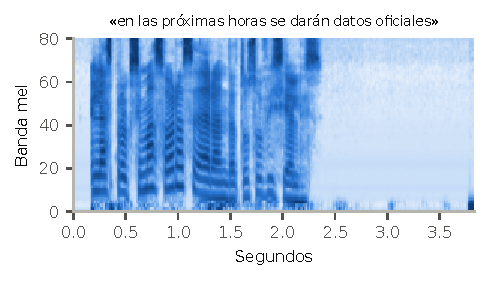
\includegraphics[width=\columnwidth]{spectrogram.pdf}
\caption{Normalized log-mel spectrogram of a test recording.}
\label{fig:spectrogram}
\end{figure}

Five experiments were trained, all selected by validation CER:
\begin{enumerate}
\item 100 Latin American recordings from scratch, with a reduced network (three GRUs of 256);
\item the same 100 recordings with augmentation;
\item pretraining on TUX only;
\item the same 100 recordings starting from the pretrained model;
\item final model: the \AudioTrain{} recordings, starting from the pretrained model.
\end{enumerate}
Augmentation combines speed perturbation ($\pm$12\,\%), noise with an SNR of 10 to 35\,dB, and SpecAugment~\cite{specaugment}. We used AdamW with warm-up, plateau, and cosine decay, gradient clipping at 5, and mixed precision, computing CTC in 32 bits.

The language model is an interpolated character 6-gram, estimated only from training texts. The values $\alpha$ = \Alpha{} and $\beta$ = \Beta{} were chosen on validation.

\subsection{Application}
Fig.~\ref{fig:architecture} summarizes the application, built with Gradio~\cite{gradio}. It has tabs for images (file, camera, or clipboard), frame-by-frame video, live camera, audio (microphone or file), and results. In video, every frame is classified and only the displayed label is smoothed with an exponential moving average. If the calibrated confidence does not reach the threshold, the application replies that it is not sure. Recordings longer than 10\,s are split at the quietest pause near the limit. Models are stored in 16 bits and nothing is sent to the Internet.

\begin{figure}[t]
\centering
\begin{tikzpicture}[
  box/.style={draw, rounded corners=2pt, align=center, font=\scriptsize, minimum height=7mm, text width=22mm},
  flow/.style={-{Latex[length=1.6mm]}}, node distance=4mm]
\node[box] (image) {Image};
\node[box, right=of image] (video) {Video or camera};
\node[box, right=of video] (audio) {Audio};
\node[box, below=of image] (crop) {224 crop and normalization};
\node[box, below=of video] (frames) {Each frame};
\node[box, below=of audio] (mel) {16 kHz and log-mel};
\node[box, below=of crop, xshift=13mm, text width=35mm] (cnn) {ResNet-50 or MobileNetV3-L};
\node[box, below=of mel] (ds) {DeepSpeech2};
\node[box, below=of cnn, text width=35mm] (cal) {Calibration, threshold, and smoothing};
\node[box, below=of ds] (beam) {Beam search + LM};
\node[box, below=of cal, text width=35mm] (class) {Class and bin};
\node[box, below=of beam] (text) {Transcription};
\draw[flow] (image) -- (crop);
\draw[flow] (video) -- (frames);
\draw[flow] (audio) -- (mel);
\draw[flow] (crop) -- (cnn);
\draw[flow] (frames) -- (cnn);
\draw[flow] (mel) -- (ds);
\draw[flow] (cnn) -- (cal);
\draw[flow] (ds) -- (beam);
\draw[flow] (cal) -- (class);
\draw[flow] (beam) -- (text);
\end{tikzpicture}
\caption{Flow of the three modalities within the application.}
\label{fig:architecture}
\end{figure}

\subsection{Origin of the Models}
No model is used as downloaded from the Internet. In vision, the only external component is torchvision's ImageNet weights, the starting point that transfer learning requires, as in the class 11 notebook. The six-class output layer is new, randomly initialized, and was trained on our data together with the unfrozen blocks (Section~\ref{sec:metodo}-C). In ResNet-50, the rest of the extractor was unchanged. In speech, no external pretrained model was used: DeepSpeech2 starts from random weights, and all of its parameters, including the TUX pretraining, were trained in this work with the CTC loss. The language model and the calibration temperature were also computed here, from the training and validation sets.

\subsection{Evaluation Protocol and Reproducibility}
The test set plays no role in training, strategy selection, calibration, or decoder tuning. The 95\,\% intervals are obtained with a 2000-replicate bootstrap, and classifiers are compared with the exact McNemar test~\cite{mcnemar}. Seed 42 was fixed in Python, NumPy, and PyTorch, although GPU operations are not bitwise deterministic. The manifests identify every example. Latency was measured on the demonstration machine (\HwCpu{}, \HwGpu{}).
